% Multi-subject/DLA EMG-based control of mechanical hands
% Castellini, Fiorilla, Sandini
%
% Submitted to Biological Cybernetics, July, 2008
%

% use option draft, final, or referee
\documentclass[twocolumn,referee]{svjour2}

\usepackage{times}
\usepackage{epsfig}
\usepackage{graphicx}
\usepackage{amsmath}
\usepackage[psamsfonts]{amssymb}
\usepackage{url}
\usepackage[pagebackref=true,breaklinks=true,letterpaper=true,colorlinks,bookmarks=false]{hyperref}

\def\RR{\mathbb{R}}
\def\NN{\mathbb{N}}
\def\xx{\mathbf{x}}
\def\yy{\mathbf{y}}
\def\ww{\mathbf{w}}

\begin{document}

\title{Multi-subject/DLA EMG-based control of mechanical hands}

\author{Claudio~Castellini \and Emanuele~Fiorilla \and Giulio~Sandini}
\institute{
  Claudio~Castellini \at LIRA-Lab, University of Genova,
  viale F. Causa, 13, 16145 Genova, Italy,
  \email{claudio.castellini@unige.it}
  \and
  Emanuele~Fiorilla, Giulio~Sandini \at Italian Institute of Technology,
  via Morego, 30, Genova, Italy,
  \email{emanuele.fiorilla,giulio.sandini@iit.it}
}

\maketitle

\begin{abstract}
  The dexterity of active hand prosthetics is limited not only due
to the limited availability of dexterous prosthetic hands, but
mainly due to limitations in interfaces. How is an amputee
supposed to command the prosthesis what to do (i.e., how to grasp
an object) and with what force (i.e., holding a hammer or grasping
an egg)? So far, in literature, the most interesting results have
been achieved by applying machine learning to forearm surface
electromyography (EMG) to \emph{classify} finger movements; but
this approach lacks, in general, the possibility of quantitatively
determining the force applied during the grasping act.

In this paper we address the issue by applying machine learning to the
problem of \emph{regression} from the EMG signal to the force a human
subject is applying to a force sensor. A detailed comparative analysis
among three different machine learning approaches (Neural Networks,
Support Vector Machines and Locally Weighted Projection Regression)
reveals that the type of grasp can be reconstructed with an average
accuracy of $90\%$, and the applied force can be predicted with an
average error of $10\%$N, corresponding to about $5$N over a range of
$50$N. None of the tested approaches clearly outperforms the others,
which seems to indicate that machine learning as a whole is a viable
approach.
%
%Notwithstanding the well-known bad conditioning of the surface EMG
%signal then, this looks highly encouraging in applying machine
%learning to enable amputees gain a fine control over advanced
%prosthetic hands, also since a surface EMG setup can be cheaply and
%easily realised and it is totally non-invasive.

\end{abstract}

\keywords{
Learning and Adaptive Systems; Rehabilitation Robotics; Physical
Human-Robot Interaction
}

%% \section{Introduction}
%% \label{sec:introduction}
%% \section{Introduction/Motivation}
\label{sec:intro}

\dropcap{A}utomatic speech recognition (ASR) is the ability of a machine
to convert human speech, coded as an audio signal, into words.
Potential applications of ASR range from human-computer interfaces
to informatics for the disabled to data mining in large speech corpora.
Despite decades of research, state-of-the-art ASR
systems still need to be trained upon very large and heterogeneous data sets
to account for speech variability.
%, or upon a single speaker's speech in controlled conditions.
And nevertheless, human beings show an excellent ability
of understanding one another's speech, independently of the speaker, the
accent, the pitch and speed, noise, etc.

Recent neuroscientific
evidence indicates that the brain motor areas responsible for producing labial
and dental phonemes are also involved in their perception; D'Ausilio et al. \cite{dausilio}
show that in a discrimination task of /b/,/p/,/d/ and /t/, trans-cranial magnetic
stimulation of the lips and tongue \emph{motor areas} creates a bias in favor
of the \emph{perception} of labials, and similarly, stimulation of the tongue
favors dentals. This suggests that motor information may be paramount for
understanding speech in humans.

Inspired by these finding, in this paper we investigate whether the knowledge of speech production in humans 
integrated into an automatic phoneme classifier improves the identification in the acoustic dimension 
of the specific behaviors of the /b/,/p/,/d/ and /t/ plosive consonants.
 
In ASR, approaches that combine explicit speech production knowledge and audio features
have been proposed (see \cite{king} for a review) as alternatives 
to the classic approach  in which the complex acoustic effects of speech production variability 
(e.g., due to speaking rate) and coarticulation (the phenomenon by which the phonetic realization of a phoneme is affected by its phonemic context) are directly and implicitly modeled in the acoustic domain.

%Although conclusions on the actual utility of speech production knowledge are somehow contradictory

By limiting our investigation on the utility of motor information to the much simpler (than ASR) task of four consonants classification\footnote{Note that a recognition task requires both segmentation of speech into phones and their classification.} we are able to relax working assumptions and avoid technical difficulties that so far have hampered a satisfactory integration of motor information into ASR systems. 

Additionally, from previous work it is not feasible to properly identify which aspects of the recognition process benefit from motor information. For example, motor knowledge may improve the modeling (and so the identification) of coarticulation effects that are seen in the training data set, but not necessarily improve the recognition of phonemes in unseen contexts, i.e., it may not necessarily improve the generalization ability of the ASR system. On the other hand the experimental setup we have designed has the main goal of investigating whether motor information improves the generalization ability of a phoneme classifier.  

%Although the integration of speech production knowledge in an ASR system often brings some improvements, %it is commonly held that the potential of speech production knowledge is far from being exhaustively exploited.  

To this end, we have focused on the automatic version of
the problem tackled in D'Ausilio et al.'s work. For each consonant,
a corresponding typical phonetic motor invariant (MI) was
identified according to basic physiology of speech;
e.g., a fast, voiced opening (plosion) of the lips for /b/, and so on.
MIs were then used to semi-automatically segment the audio/motor data found in a
database of speech/motor trajectories recorded from $6$ subjects.

Subsequently, a simple regression method (namely, a feed-forward neural network) was employed
to build an Audio-Motor Map (AMM), which converts audio features of the isolated segment to
features of the related MI. On an abstract level, an AMM is a mathematical proxy of a mirror
structure \cite{umilta-01}, reconstructing the distal speaker's speech production act while
listening to the related piece of speech.

To test the approach, we have devised three experiments involving a 
classifier in the form of a Support Vector Machine \cite{BGV92}. We wanted to check whether
the use of MI-based features, either those recorded in the database (the ``real''
motor features) or the AMM-reconstructed ones (a more ecological scenario),
could improve the classifier's performance. Our results show that this is the case,
especially when the classifier is trained on incomplete data sets such as 
per-speaker (e.g., training on speakers $1,2,3$ and testing on $4$) and
per-coarticulation(e.g., training on /ba/, /be/, /bi/, /bo/ and testing on /bu/); or when noise is added,
in which case motor features significantly help classification, even when added to a
state-of-the-art set of audio features about $20$ times larger than that extracted
from the MIs.

\subsection{Related Work}

It is known since the Sixties \cite{liberman1} that the audio signal of speech
cannot be effectively segmented down to the level of the single phoneme,
especially as far as stop consonants such as bilabial plosives
are concerned; in particular, their representations in the audio domain are
radically different according to the phoneme which immediately follows.
It remains an open question then, how humans can
distinctly perceive a common phoneme, e.g.,/b/ in  /ba/ and /bi/, since they
apparently have access to the speaker's audio signal only.

The explanation put forward by the so-called motor theory of speech perception
(MTS, \cite{liberman2,galant}) is that, while perceiving sounds,
humans reconstruct \emph{phonetic gestures}, the physical acts of
producing the phonemes, as they were trained since birth to associate
articulatory gestures to the sounds they heard. 

Even ignoring the motor theory of speech perception the use of speech production knowledge is appealing in that the coupling of articulatory and audio streams allows for explicit models of the effects of speech production phenomena (e.g., coarticulation) on the acoustic domain. These effects cannot be precisely modeled (e.g., when the phoneme /a/ affects the phonetic realization of /b/ in /ba/?)  or modeled at all (e.g., what happens when I utter a /o/ with exaggeratedly open jaw?) when the phonemic stream is directly mapped onto the acoustic dimension as in the standard approach to ASR.  

Different solutions have been proposed to integrate speech production knowledge into an ASR system and different types of speech production information has been used, ranging from articulatory measurements (see \cite{zlokarnik,stephenson,wrench}, for example) to symbolic non-measured representations of articulatory gestures that "replicate" a (symbolic) phoneme into all its possible articulatory configurations\footnote{Articulatory configurations are configurations of the positions of the phonetic articulators} (see \cite{richardson, livescu}, for example).
 
   
%One possible reason why ASR is so difficult is then that
%machines have in general no access to the motor representation of the
%audio signal they are supposed to understand. We hypothesize that motor 
%information might help ASR, especially when tests on different speakers and different
%coarticulations are performed: for example, when training on subject $A$ and
%testing on subject $B$, or when training on pseudo-words such as /ba/, /bi/,
%/be/ and then testing for the presence of /b/ in /bo/, /bu/ or even /br/.

Although some studies have shown increased word recognition accuracy when including speech production knowledge in ASR, it is commonly held that the potential of speech production knowledge is far from being exhaustively exploited. Limits of current approaches include: the use of the phoneme as basic unit (as opposed to articulatory configuration, for example) which appears to be too "coarse", especially in the context of spontaneous spoken speech 
%where coarticulation effects are more frequent and marked
;and  the lack of a mechanism that accounts for the different importance of articulators in the realization of a given phoneme (e.g., in the generation of phoneme /b/ lips are critical, i.e., important, while tongue is non-critical).

The traditional approach in which the speech signal is segmented into phones, often referred to as "beads on a string" approach, poses problems to an accurate modeling of spontaneous speech where coarticulation phenomena such as phone deletion or assimilation (where a phone assimilates some articulatory gestures of the preceding/following phone), are frequent and not always predictable and call for finer-grained basic units (see \cite{ostendorf})). To partly make-up for such limitation we propose an alternative approach where, instead of segmenting the audio stream looking at audio features only and then observing the articulatory gestures within the identified phones, we give priority to the motor information in that speech is segmented by searching for phone-specific patterns of the (critical) articulatory gestures.

%Concerning the necessity of a phoneme dependent distinction between critical and non-critical articulators we do not 
%Traditionally (e.g., \cite{bourl,salvi}), the audio speech signal is segmented with a
%fixed-length Hamming window, usually 20ms. long. The resulting sequence
%is then analysed in the frequency or cepstral domain and the
%resulting coefficients are used as features for a classification system.
%One negative aspect of this approach is that it
%neglects the qualitative overall characteristics of the
%phoneme being uttered: depending on the speed of the speech, a consonant
%can have different lengths and, by using the above approach, global
%information about it is lost (see \cite{ostendorf}, where this approach is
%dubbed ``beads-on-a-string''). Nevertheless, as far as we know, there is
%so far no widely accepted alternative method for speech segmentation,
%if the audio signal is the only one available. One attempt, but not based
%upon articulatory data atl all, appears in \cite{bourlard}.


During recognition, articulatory gestures have to be recovered 
from audio information as audio is the only signal available.
Reconstruction of articulatory features has been attempted since a long
time, but in most cases it is not derived from articulatory \emph{data}
gathered from human subjects. One pioneeristic case is that of Papcun
et al. \cite{papcun} where the AMM is carried out by a Multilayer Perceptron.
Our procedure for building the AMM is deeply inspired by this work.
%By using a Multilayer Perceptron we implicitly assume that all articulators have the same importance and that the AMM is a %one-to-one mapping.   
%Papcun et al. \cite{papcun} observed that non-critical articulators have higher variance (in terms of position) than critical %articulators. 
The Multilayer Perceptron tries to carry out the best recovery of all articulatory gestures while more emphasis to the recovery of the gestures of the critical articulators should be given to the detriment of the non-critical articulators, which have higher variance (in terms of position, see \cite{papcun,rose}). Although we do not address this issue, the simple fact that we only consider two articulators alleviates a problem that would be otherwise far more relevant if all articulators were taken into account\footnote{The higher variance of the non-critical articulators is the main cause that makes AMM a one-to-many mapping: different articulatory configurations result in the same acoustic realization. Solutions to properly address this "ill-posed" nature of the AMM have been proposed by Richmond et al. \cite{richmond} and Toda et al. \cite{toda}. }.

%and subsequently Korin Richmond's work
%\cite{richmond2002,richmond2007} who have been able to reconstruct point-by-point
%the trajectories of articulators from the audio signal to a remarkably low
%error rate. The procedure for building the AMM is deeply inspired by their
%work.

Interestingly, the idea of using information about the mechanisms involved in the production of a human action to improve its classification/recognition (in a domain different from the production domain) has not only been applied in the context of speech recognition. For example Metta et al. \cite{metta-06} and Hinton \cite{hinton-2006} 
have shown that articulatory data can improve classification accuracy in automated hand action classification.

%TODO  
% Transferring the method to speech perception seems
% like a natural choice.


%% \section{Materials and Methods}
%% \label{sec:m&ms}

%% \subsection{Experimental Setup and Design}
%% \label{subsec:setup}
%% \begin{figure*}[!t] \centering
  \begin{tabular}{ccc}
    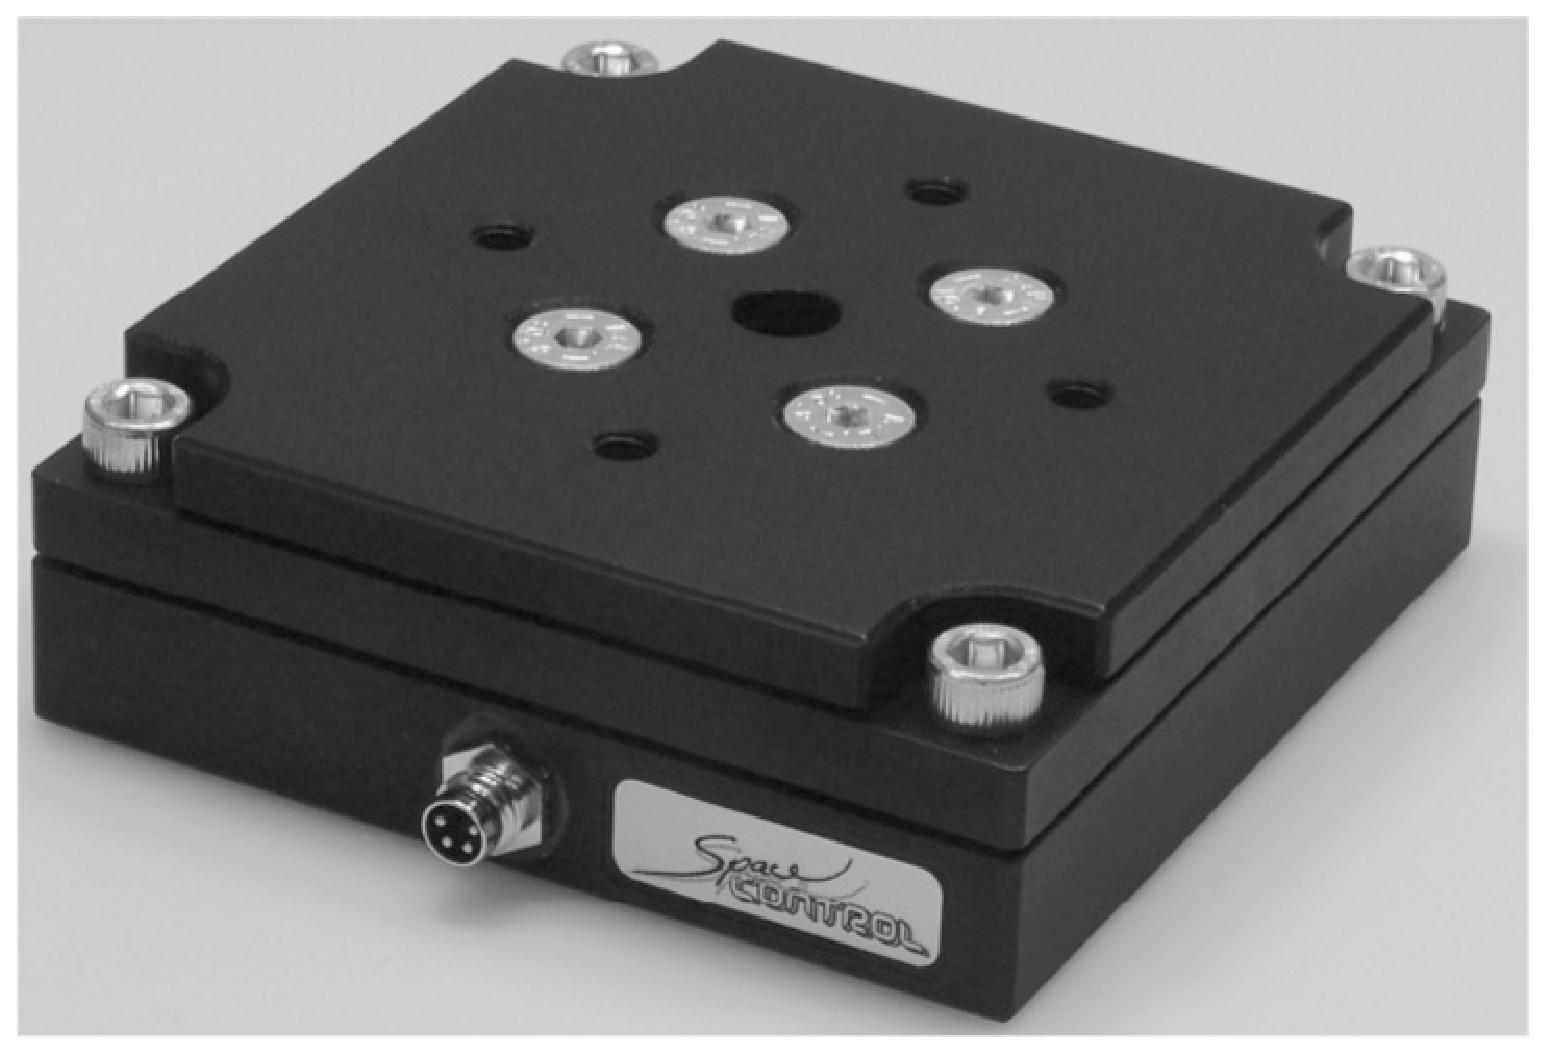
\includegraphics[height=0.16\textheight]{figs/OFTS} &
    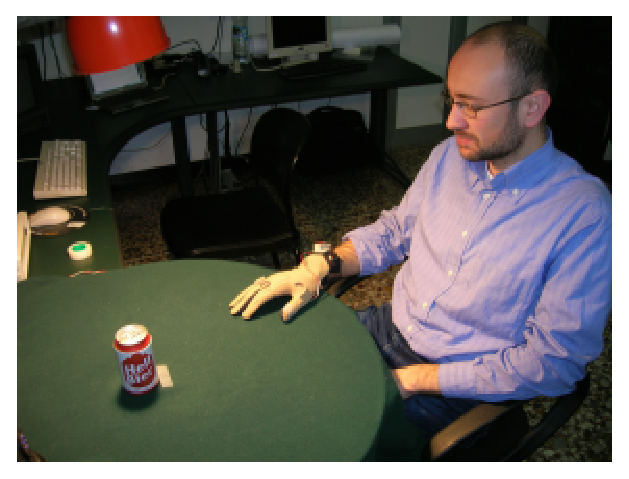
\includegraphics[height=0.16\textheight]{figs/setup} &
    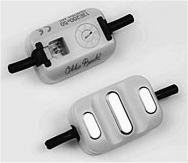
\includegraphics[height=0.16\textheight]{figs/ottobock} \\
    $(a)$ & $(b)$ & $(c)$ \\
  \end{tabular}
  \caption{The experimental setup. $(a)$ The SpaceControl OFTS
    force/torque sensor, large face up. $(b)$
    The arm of the subject with the EMG electrodes fitted and held in
    place by elastic bands. Electrode cables are wired in a box and
    then directed to a National Instruments PCI-6023E analogic/digital
    conversion card (not shown). $(c)$ An Otto Bock 13E200=50
    surface EMG electrode, with the amplification gauge (upper part of
    the Figure) and the three metallic contacts (lower part).}
  \label{fig:setup}
\end{figure*}

\subsubsection{General setup description}

The experiment consisted of freely, repeatedly grasping a SpaceControl
OFTS force/torque sensor \cite{ofts} orthogonally to its large face
(see Figure \ref{fig:setup} $(a)$). Four different ways of pressing
were allowed: opposing the thumb and index, the thumb and middle, the
thumb and ring or the thumb and all other fingers. The speed and force
was intentionally left to the subject's will. Four force sensing
resistors (FSRs) were applied on the subject's hand fingertips (thumb,
index, middle and ring), in order to be able to detect which grasp
type was used at each instant of time. At the same time, $10$ forearm
surface EMG electrodes were applied to the subject's forearm, held in
place by elastic bands, in order to gather information about the
muscle activation (see Figure \ref{fig:setup} $(b)$).

Numerical data from the EMG electrodes, FSRs and OFTS were gathered at
the fastest sampling rate we could obtain, that is, $256$Hz, using a
National Instruments DAQ PCI-6023E analogic/digital conversion card
\cite{nidaq}, mounted on a fast PC equipped with Windows XP.

\subsubsection{EMG signal and electrode placement}
\label{subsubsec:electrodes}

The $10$ EMG electrodes were applied to the subject's right forearm,
held in place by elastic bands. The electrodes were
double-differential Otto Bock 13E200=50 models (\cite{ottobock}, see
Figure \ref{fig:setup} $(c)$), each one gifted with an amplification
gauge ranging from $2000$ to $100000$ times. Initial qualitative
experiments revealed that a safe setting for the amplification gauge
was in the middle of the range, corresponding to about $14000$
times. This is in agreement with the EMG signal amplitude predicted in
the related literature (see, e.g., \cite{deluca}), that is about $100
\mu V$ on average: the voltages our DAQ card read ranged from $0V$ to
about $2.5V$.

Six of the electrodes were placed in pairs along the lower face of the
forearm, whereas four of them were applied in pairs on the upper
face. The initial positioning of the electrodes was chosen in order
for them to lie approximately on top of the muscles which elicit
finger movements; the precise placement was done following the
description in \cite{smagt}, which proved to be optimal for Support
Vector Machine classification of hand postures.

As far as the EMG signal is concerned, it must be remarked that it is
subject to remarkable changes depending on, at least, four orders of
factors:

\begin{enumerate}

  \item \emph{inter-subject variability.} All forearms are different
    from one another in shape, size and power.

  \item \emph{arm posture.} Besides finger movements and grasping, the
    forearm muscles are also involved in the motion of the arm. The
    EMG signal is therefore likely to change if the forearm is moved
    during signal acquisition, for example when switching from
    pronation to supination, or simply while walking around. Even
    raising the shoulder to lift the forearm from the table will
    result in remarkable signal changes.

  \item \emph{electrode displacement.} The intensity and quality of
    the EMG signal depends upon a correct placement of the electrode
    over a muscle. In principle, each electrode should be placed over
    a single muscle, precisely on top of the muscle belly, halfway the
    length of the muscle, and always exactly in the same place.
    Displacing the electrodes will alter the signal, and beside that,
    a precise placement is essentially impossible when dealing with
    surface forearm EMG.

  \item \emph{muscle fatigue.} As the muscles are used more and more,
    continually, fatigue changes the RMS of the EMG signal, calling
    for continual adaptation, at least over a reasonable set of
    different fatigue conditions.

\end{enumerate}

Problems $1$ and $2$ have been for now neglected by concentrating on
one subject only, male, aged $35$ and fully able-bodied, instructed to
keep the arm still and relaxed on a table in a confortable position,
with the palm orthogonal to the plane of the table. See the Discussion
Section for more about these issues.

As far as muscle fatigue and electrode displacement are concerned,
electrodes \emph{cannot} be expected to exactly lie in the very same
position every time the prosthesis is used; moreover, in a preliminary
round of experiments, muscle fatigue was clearly perceived by the
subject during the experiment. In this framework, the only possibility
to overcome these problems is to explicitly take them into account,
gathering enough data to be able to train the machine under different
conditions of electrode displacement and muscular fatigue.

We then organised the experiment as follows: the subject was
instructed to continually grasp the sensor over a period of time of
three to four minutes; then he was allowed to rest for about two
minutes. This was called a \emph{session}. It was expected that muscle
fatigue would appear already during one session. Three sessions were
gathered without taking the elastic bands off the subject's forearm,
in order \emph{not} to have electrode displacement within such a set
of sessions, that we called a \emph{group}. After each group, the
electrodes and bands were removed and the subject was allowed for a
much longer period of rest, ranging from half an hour to one
hour. During resting in-between groups, the subject could get back to
his normal muscular activity.

Five groups were then gathered during one day; and this procedure was
entirely repeated during another day. This procedure would allow us to
examine a relevant amount of data, gathered along a relatively long
period of time and under different conditions of muscle fatigue
(within one session) and electrode displacement (between groups). As
an example, Figure \ref{fig:drift}, pane $(a)$, shows the typical
electrode output during a session (moving average over about $10$
seconds). One can notice strong low-frequency components due to muscle
fatigue.

Spectral analysis of the EMG signal revelaed that all relevant
information is limited to $10$Hz (damping of $-30$dB at that
frequency), therefore sampling at $256$Hz proved to be a large
overshoot. We will employ this fact later on.

\begin{figure}[!ht] \centering
  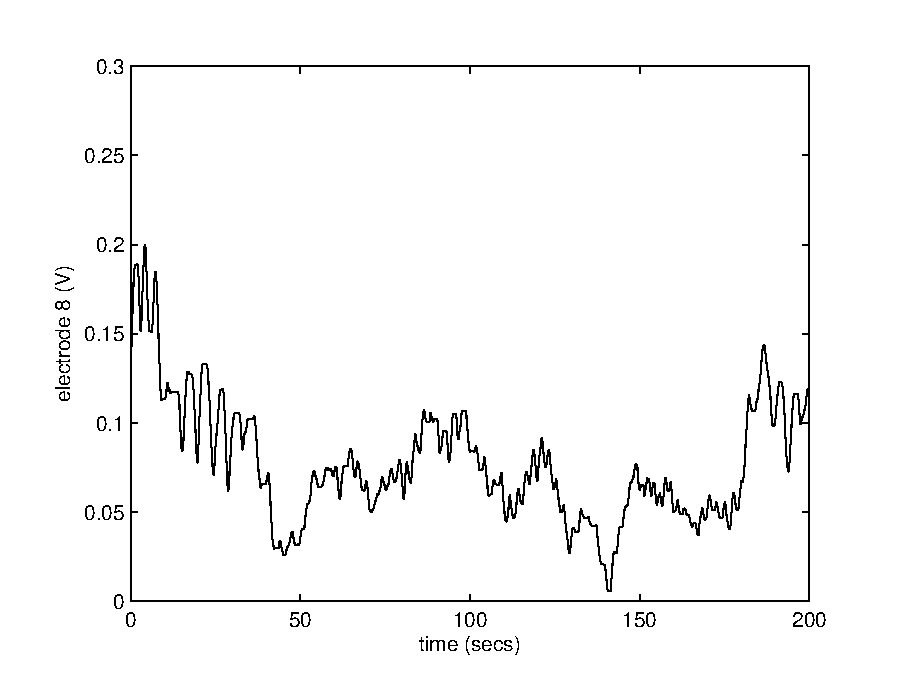
\includegraphics[width=0.45\textwidth]{figs/el8_movingAvg_s1}
  \caption{Typical behaviour of an electrode signal over a
    session (moving average over about $10$ seconds). Drifting can be
    clearly seen in the signal, due to muscle fatigue.}
  \label{fig:drift}
\end{figure}

\subsubsection{Force applied during the grasp}

The OFTS force/torque sensor would output a (negative) integer
numerical value ranging from $0$ to about $-5000$, expressed in
(negative) fiftieths of a Newton. After normalisation, the range of
the applied force would then be between $0N$ and $100N$, with a
resolution of $0.02N$. Linearity of the sensor is guaranteed, and was
anyway manually verified.

\subsubsection{Type of grasp}

The voltage values output by the $4$ FSRs applied onto the subject's
fingertips were monitored in order to understand which kind of grasp
the subject was applying to the sensor. A threshold was experimentally
decided, above which the finger would be defined \emph{in contact}
with the sensor. Using this technique, for each instant in time one of
five possible categories was established: $0$, no action; $1$, grasp
by opposing the thumb and index finger; $2$, opposing thumb and
middle; $3$ thumb and ring; and lastly $4$, grasp by opposing the
thumb and all other fingers.

It must be remarked here that the EMG signal would be altered
immediately at the onset of finger movement, which our setup was
unable to detect. This would result in potential wrong EMG values for
category $0$. Moreover, the FSRs have been experimentally determined
to suffer from a remarkable hysteresis effect, that is, they will
indicate slightly different voltage while pressing and releasing; this
is due to small rubber ends glued on top of the sensor surfaces, which
aid grasping by raising the static friction coefficient. Hysteresis is
also supposed to somehow degrade the quality of the learning. Because
of these factors we would never expected a close-to-$100\%$
classification accuracy, nor a perfect reconstruction of the applied
force. A better setup is currently being studied, which would avoid
these effects. Again, see the Discussion for more about this issue.


%% \section{Experimental Evaluation}
%% \label{sec:exp}

%% \section{Discussion and Conclusions}
%% \label{sec:discussion}
%% Our experimental results, performed on a large data set of about
$153000$ samples, clearly show that the Online Uniformisation
procedure can be used uniformly to obtain dramatically smaller
training sets with no \emph{qualitative} loss of information; in other
words, as more of the input space is sampled, OU keeps the training
set up-to-date and small. OU sets will result in fast and accurate
models of the sought-for EMG-to-hand map. Remarkably, OU works fine
for both grasp classification and force regression, and with all three
different machine learning approaches. Moreover, OU is extremely
simple, being nothing more than an online check of Euclidean distance
in the input space. This check is done so far by considering the new
sample's distance from all samples in the current training set, and
therefore could become unfeasibly heavy as the set grows; but the same
check can be done in constant time using an algorithmic optimisation,
such a hash table.

We believe this is the first step toward the real application of
machine learning to an EMG-driven adaptive, dexterous hand
prosthesis. Let us consider the problems outlined in Subsection
\ref{subsubsec:electrodes}: in this paper we have solved problems
$3$ and $4$. Now, since OU lets us obtain good accuracy with extremely
small training sets, it is not too far-fetched to say that the
solution of problem $2$ is at hand --- in principle, the changing arm
posture can be taken into account simply by sampling more of the input
space. Problem $1$ is, really, of lesser interest, since one patient
only is supposed to ever wear a prosthesis.

As far as force regression is concerned, the results presented above
are, to the best of our knowledge, totally novel. Surprinsingly,
regression from the forearm surcafe EMG signal to the force applied by
the hand had never been attempted before. Given the good performance
obtained by our models, we claim that the relationship between the EMG
signal and the force has been captured by the models, under variable
conditions of muscle fatigue (within one session) and electrode
displacement (within sessions belonging to different groups).

All in all, in this paper we have presented a machine learning
approach to joint classification of grasping and regression on the
applied force, using forearm surface electromyography. The approach is
totally non-invasive, easy to set up and use and it can be applied
from scratch with no previous knowledge of the problem. The Online
Uniformisation procedure can be used to incrementally build a training
set which will result in small and accurate models of the problem.

Our experiments, carried out using a Support Vector Machine with
Gaussian kernel, a Neural Network with sigmoidal activation function
and Locally Weighted Projection Regression, indicate that the approach
achieves, using a training set of about $1800$ samples on a total of
$153000$ (for $d=021$), an average accuracy of around $90\%$ in
classification of grasp types and a normalised root MSE of $7.89\%$ in
prediciton of the force applied during the grasp. Of the tested
approaches, SVM is marginally better than the others, especially when
larger training sets are used. The OU procedure is able to find as
small a training set as $77.4$ samples on average (out of $153000$),
which will still result in a SVM having an NRMSE of $12.12\%$.

Future work can be divided in three steps: firstly, problem $2$ of 
\ref{subsubsec:electrodes} must be taken into account by gathering
more samples, possibly with a more sophisticated EMG/force sensing
setup. Secondly, once a stable model has been built, the actual
position/force control of a mechanical hand must be realised. And
thirdly, in the medium-to-long term, we plan to implant the hand on a
disabled person with extensive experiments to test the real usability
of the proposed approach.


%\section*{Acknowledgments}

{\small
\bibliographystyle{spbasic}
\bibliography{paper}
}

\end{document}
